\documentclass{bioinfo}
\copyrightyear{2012}
\pubyear{2012}

\usepackage{subfig}
\usepackage{listings}
\usepackage{ifthen}

\lstset{language=Java,
morendkeywords={String, Throwable}
captionpos=b,
basicstyle=\scriptsize\ttfamily,%\bfseries
stringstyle=\color{darkred}\scriptsize\ttfamily,
keywordstyle=\color{royalblue}\bfseries\ttfamily,
ndkeywordstyle=\color{forrestgreen},
numbers=left,
numberstyle=\scriptsize,
% backgroundcolor=\color{lightgray},
breaklines=true,
tabsize=2,
frame=single,
breakatwhitespace=true,
identifierstyle=\color{black},
% morecomment=[l][\color{forrestgreen}]{//},
% morecomment=[s][\color{lightblue}]{/**}{*/},
% morecomment=[s][\color{forrestgreen}]{/*}{*/},
commentstyle=\ttfamily\itshape\color{forrestgreen}
% framexleftmargin=5mm,
% rulesepcolor=\color{lightgray}
% frameround=ttff
}

% MACROS:

\newcommand{\TODO}[1]{\textcolor{red}{\textbf{#1}}}
\newcommand{\AbstractDESSolver}{\texttt{Abstract\-DES\-Solver}}
\newcommand{\OverdeterminationValidator}{\texttt{Overdetermination\-Validator}}
\newcommand{\SBMLinterpreter}{\texttt{SBML\-interpreter}}
\newcommand{\FirstOrderSolver}{\texttt{First\-Order\-Solver}}
\newcommand{\AbstractIntegrator}{\texttt{AbstractIntegrator}}
\newcommand{\MultiTable}{\texttt{Multi\-Table}}
\newcommand{\Block}{\texttt{Block}}

\hyphenation{
  % TODO hypens for regular words
}

% some nice colors
\definecolor{royalblue}{cmyk}{.93, .79, 0, 0}
\definecolor{lightblue}{cmyk}{.10, .017, 0, 0}
\definecolor{forrestgreen}{cmyk}{.76, 0, .76, .45}
\definecolor{darkred}{rgb}{.7,0,0}
\definecolor{winered}{cmyk}{0,1,0.331,0.502}
\definecolor{lightgray}{gray}{0.97}

\begin{document}
\firstpage{1}

\title[SBML Simulation Core Library]{Simulation Core Library: the Java
library for numerical computation in systems biology} \author[Dr\"ager
\textit{et~al.}]{%
Andreas Dr\"ager\,$^{1,*}$, Roland Keller\,$^{1}$, 
Alexander D\"orr\,$^{1}$,
Akito Tabira\,$^{2}$,
Akira Funahashi\,$^{2}$,
\TODO{%
Michael J. Ziller\,$^{3}$
Nicolas Rodriguez\,$^{4}$,
Nicolas Le Nov\`{e}re\,$^{4}$} and
Andreas Zell\,$^1$\footnote{to whom correspondence should be addressed}}
\address{$^{1}$Center for Bioinformatics Tuebingen (ZBIT), University of
Tuebingen, T\"ubingen, Germany\\
$^{2}$Keio University, Graduate School of Science and Technology, Yokohama,
Japan\\
\TODO{%
$^{3}$Department of Stem Cell and Regenerative Biology, Harvard University,
Cambridge, MA, United States\\
$^{4}$European Bioinformatics Institute, Wellcome Trust Genome Campus,
Hinxton, Cambridge, UK\\}}

\history{Received on XXXXX; revised on XXXXX; accepted on XXXXX}

\editor{Associate Editor: XXXXXXX}

\maketitle

\begin{abstract}

\section{Motivation:}
Following the aim to make biological phenomena predictable, modeling, 
simulation, and computer analysis of biological networks has become an integral
part of modern biological research. XML-based standard description languages
such as the Systems Biology Markup Language (SBML) or CellML specify rich sets
of methods for the interpretation of biological network models in terms of a
differential equation system with additional events and rules.
Although libraries for reading and manipulating the information content of
these XML-based languages are available, a multiple-purpose and 
efficient numerical solver library that has been designed with respect to the
requirements of biological network models is a crucical prerequisite. 
The vast majority of available solvers for these systems is either
part of a larger software suite and can therefore not be easily integrated into
custom programs, or implemented in programing languages, which are either
platform-dependent or even require a commercial license for their
execution.

\section{Results:}
The Simulation Core Library provides a large
collection of numerical solvers and a sophisticated interface hierarchy for the definition of custom
differential equation systems. It is entirely
implemented in Java\texttrademark{} without the necessity to
include any platform-dependent wrappers or libraries, does not depend on any
commercial library, and can be used on every operating system for which a Java
Virtual Machine is available.
It already includes an efficient and exhaustive implementation of methods to
interpret the content of models encoded in the SBML based on the JSBML project.
To demonstrate its
capabilities, it has been benchmarked against the entire SBML Test Suite and
also been used to simulate all models of the BioModels.net database.

\section{Availability:}
Source code, binaries, and documentation for SBML Simulation Core can
be freely obtained under the terms of the LGPL 3.1 from the website
\href{http://www.cogsys.cs.uni-tuebingen.de/software/SBMLsimulator}{http://www.cogsys.cs.uni-tuebingen.de/software/SBMLsimulator}.

\section{Contact:}
\href{mailto:andreas.draeger@uni-tuebingen.de}{andreas.draeger@uni-tuebingen.de}

\section{Supplementary information:}
% TODO: Provide additional material
Supplementary data is available at Bioinformatics online.

\end{abstract}

\section{Introduction}

The modeling language SBML (Systems Biology Markup Language,
\citealt{Hucka2003}) constitutes an important \emph{de facto} standard for the
exchange of biochemical network models.
SBML defines a set of data structures and provides rules about how to interpret
and simulate these kinds of models.

A model stored in SBML may combine an ordinary differential equation system,
which is the basis for numerical simulation, with additional elements such as
rules and events.  These elements further influence the system. For instance,
an event takes place if a certain trigger condition becomes true. Whenever this
happens, event assignments may change the values of model components, such as
parameter values or compartment sizes. Rules can directly assign new values to
their objectives, e.g., the concentration of a reacting species.

In many cases, model parameters with uncertain values, such as kinetic
constants, need to be estimated using heuristic optimization procedures in
order to minimize the distance between model output and experimental
measurement data.

For model building, simulation, and parameter calibration processes,
appropriated software implementations are indispensable. There are several
larger tools with a graphical user interface written in Java\texttrademark{}, C
or MATLAB that fulfil those important requests:
\citep{Loew2001}, \citep{Myers2009}, \citep{Maiwald2008}, \citep{Hoops2006}, 
\citep{SBT_Schmidt2006}, \citep{Bergmann06}.
But it is difficult to integrate the contained simulation routines in other programs.
The SBML ODE Solver Library \citep{Machne2006}, which is written in C and based
on the libSBML library \citep{Bornstein2008},  provides such a simulation
routine. The SUNDIALS package is used for solving the differential equation system given in the model.

In contrast to that we here present a platform-independent simulation API in
Java that interprets the content of such a model and predicts the dynamic behavior of the model�s
components. It is the first simulation routine which is based on the
Java\texttrademark{} library JSBML \citep{Draeger2011b}, a specifically
developed data structure to read and write models from and into SBML files and
to deal with their structure in memory. The API contains an interpreter for the
SBML model and several different ODE solvers. The generic library is completely
decoupled from any graphical user interface and can hence easily be integrated
as an API (Application Programming Interface) into third-party programs under
the terms of the LGPL Version 3.
\TODO{Describe this as a potential application.}
The SBML simulation core library has already been integrated into the widely
used program CellDesigner version 4.2 \citep{Funahashi2003} as an internal simulation
library.
\TODO{Mention the stand-alone application SBMLsimulator.}
%Secondly, a graphical and command-line user interface that provides
%a connection to the heuristic optimization framework EvA2 \citep{Kron10EvA2}.
% The combination of SBMLsimulator and EvA2 \citep{Kron10EvA2} estimates the values of all parameters with
%respect to given time-series of metabolite or gene expression values. 

\begin{methods}
\section{Implementation}
\begin{figure*}
\centerline{
  \subfloat[Solvers.]{
    \label{fig:Solvers}
    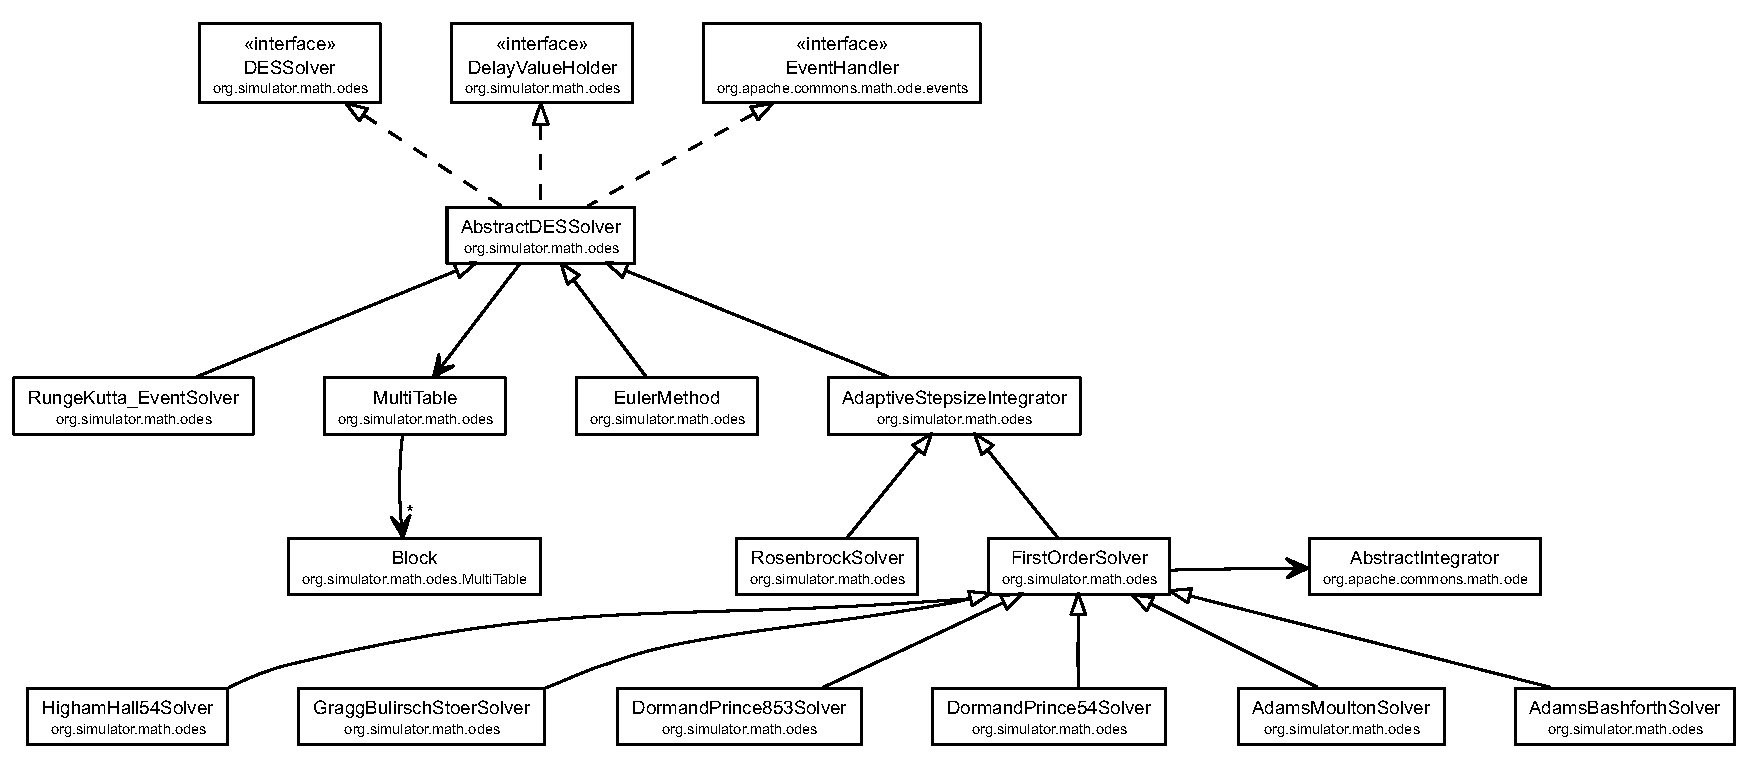
\includegraphics[width=.5\textwidth]{img/Solvers.pdf}
  }
  \hfill
  \subfloat[Differential equation systems.]{
    \label{fig:DESystems}
    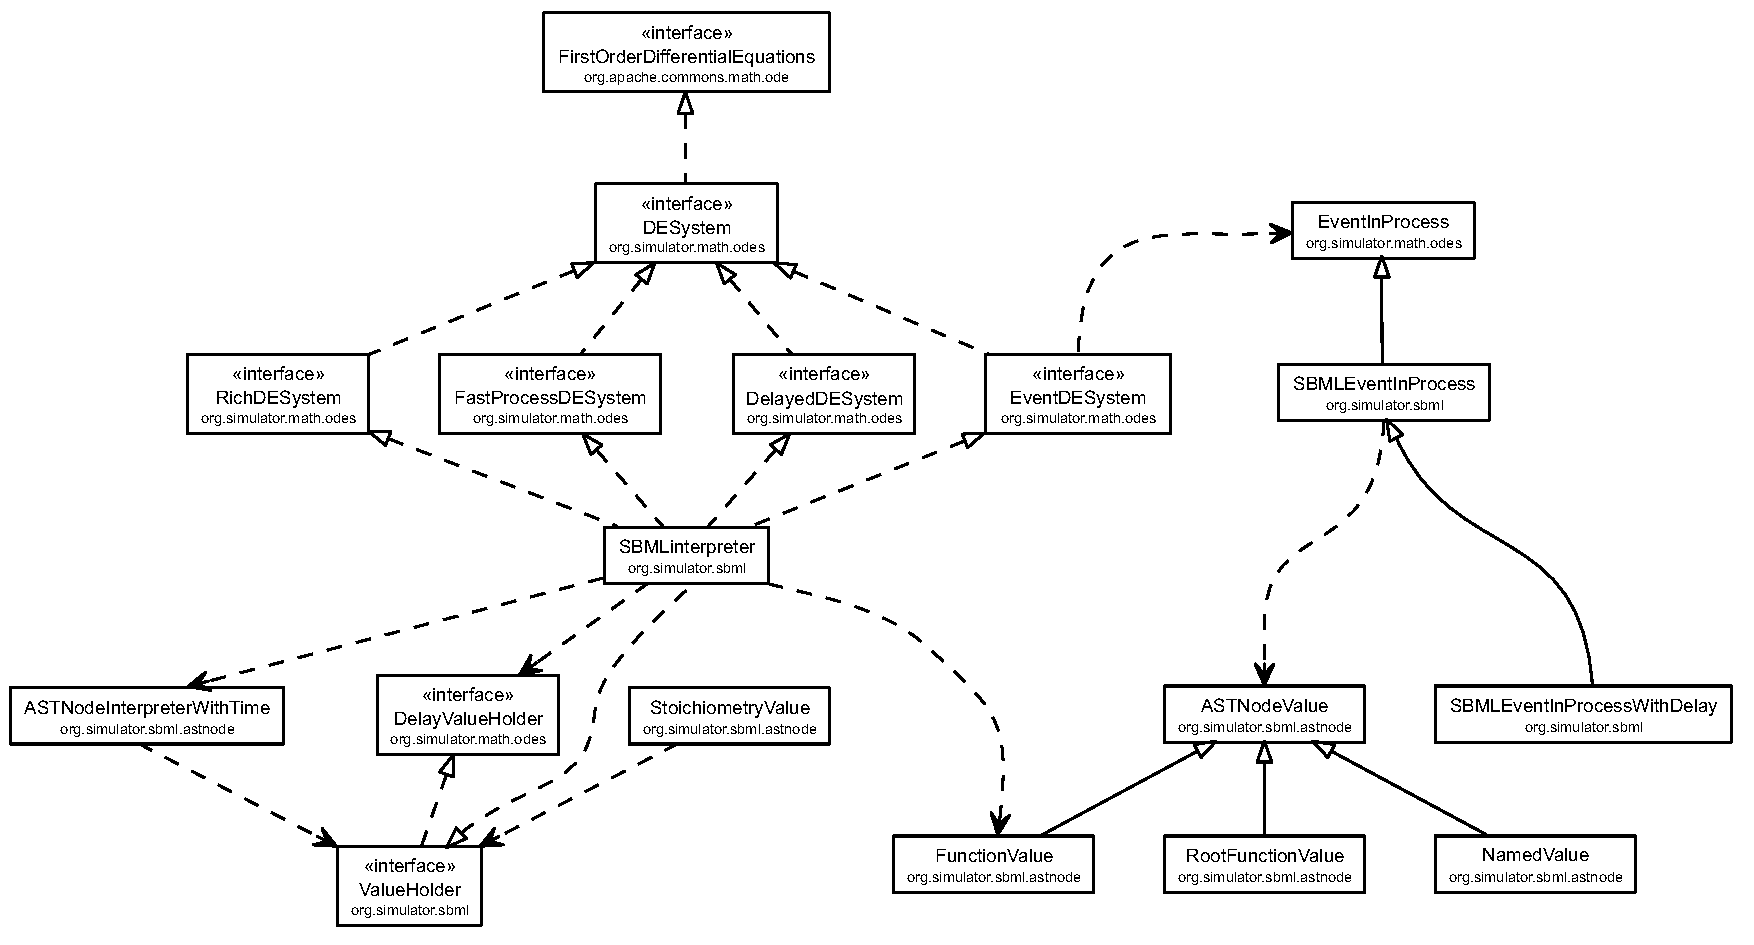
\includegraphics[width=.5\textwidth]{img/SBMLInterpreter.pdf}
  }
}
\caption[Architecture of the Simulation Core Library]{Architecture of
the Simulation Core Library (slightly simplified). Numerical methods are
strictly separated from differential equation systems. Fig.~\ref{fig:Solvers} displays the unified type
hierarchy of all numberical integration methods, which are currently part of the
library, including solvers from Apache Commons Math library and Rosenbrock's
method. The class \MultiTable{} stores the results of a simulation within its
\Block{} data structures. Fig.~\ref{fig:DESystems} shows the interfaces that
define several special types of the differential equations to be solved by the
numerical methods. This abstract description makes it possible to describe
various types of differential equation systems without directly linking it to a
particular type of biological networks. The class \SBMLinterpreter{} implements
all of these interfaces with respect to the information content of a given SBML
model. The interpreter causes the main run-time of the integration procedure.
This is why efficient and clearly organized data structures are required to
ensure a high performance of the overall library. The interpretation of SBML
models is therefore organized in the evaluation of events and rules, the
computation of stoichiometric information, and the computation of the current
values of all model components (such as species and compartments).
In this way it is possible to pass an instance of an interpreter for a
particular model system, such as SBML or CellML, to any available solver.}
\label{fig:Architecture}
\end{figure*}
In this API a large collection of differential equation solvers and an
interpreter for SBML are provided. The solvers and the interpretation of SBML
are independent of each other.

All the solver classes are derived from the abstract class \AbstractDESSolver.
The Eulerian and the Runge-Kutta solver are very fast, but not suitable
for some differential equation systems. Several solvers of the Apache Commons
Math library are integrated with the help of wrapper classes. The Rosenbrock
solver \citep{Kotcon2011} is slower than the other solvers, but it can be used
for solving stiff differential equation systems.

The class \SBMLinterpreter{} stores and processes a given SBML model. For a given
value of the ODE system and a given time it returns the current set of
derivatives of the variables. It is connected to an efficient
interpreter for MathML expressions that are contained in kinetic laws, rules
and events. The nodes of the syntax tree of those expressions depend on the
current simulation time and the given values of the ODE system. If the time or
any of these values has changed, the value of the node has to be recalculated.
At the beginning of the simulation the syntax trees of all kinetic laws, rules
and events are restructured and merged to one large tree that contains
equivalent nodes only once. This leads to a decreasing computation time during
the simulation.

An extremely important aspect in the interpretation of SBML models is the
determination of the exact time at which an event occurs, as this can have a
high influence on the precision of the values of the system variables. We have
therefore adapted the Rosenbrock solver, which is an integrator with an adaptive
step size, to a very precise timing of the events.

Algebraic rules are transferred to assignment rules before the simulation: One
of the variables contained in an algebraic rule is chosen as the variable of the
created assignment rule and the equation is solved by this variable. The
\OverdeterminationValidator{} in JSBML helps to ensure that no conflicts occur
between any of the chosen variables.

The simulation algorithm now proceeds as follows: In each time step the ODE
solver gets the current set of values of the variables as its initial values and
calculates the values for the next time point. After that events
and rules are processed, that can change the values. The calculated values are
then the initial values for the next time step. The event processing of the
Rosenbrock solver is different from that of the other solvers, as it
is directly integrated in the solver and influences the adaptation of its step
size. This makes the processing of the events extremely precise.

\end{methods}

\section{Results}
Our implementation has been successfully tested with the SBML test suite (see
\href{http://sbml.org/Software/SBML_Test_Suite}{http://sbml.org/Software/SBML\_Test\_Suite})
and the models of the biomodels.net database: With the Rosenbrock solver all
models of the test suite are simulated correctly and all but three models of the
\href{http://biomodels.net}{BioModels.net} database \citep{Novere2006a}
\TODO{can be simulated in acceptable time}.

%\begin{table}[!t]
%\processtable{This is table caption\label{Tab:01}}
%{\begin{tabular}{llll}\toprule
%head1 & head2 & head3 & head4\\\midrule
%row1 & row1 & row1 & row1\\
%row4 & row4 & row4 & row4\\\botrule
%\end{tabular}}{This is a footnote}
%\end{table}


%%%%%%%%%%%%%%%%%%%%%%%%%%%%%%%%%%%%%%%%%%%%%%%%%%%%%%%%%%%%%%%%%%%%%%%%%%%%%%%%%%%%%
%
%     please remove the " % " symbol from \centerline{\includegraphics{fig01.eps}}
%     as it may ignore the figures.
%
%%%%%%%%%%%%%%%%%%%%%%%%%%%%%%%%%%%%%%%%%%%%%%%%%%%%%%%%%%%%%%%%%%%%%%%%%%%%%%%%%%%%%%

\section{Conclusion}
The SBMLsimulator API is an efficient Java tool for the simulation of
differential equation systems given in SBML. It can be easily integrated in
larger applications, which display the simulation results or optimize some
parameters of ODE models. 
With the given program structure the support of other model formats (e.g.,
CellML, \citealt{Lloyd2004}) can be added by only implementing an interpreter
for each format.


\section*{Acknowledgement}

The authors are grateful to Beky Kotcon, Samantha Mesuro, Daniel Rozenfeld, Anak
Yodpinyanee, Andres Perez, Eric Doi, Richard Mehlinger, Steven Ehrlich, Martin
Hunt, George Tucker, Peter Scherpelz, Aaron Becker, Eric Harley, and Chris
Moore, Harvey Mudd College, Claremont, California, USA, for providing an
Java implementation of Rosenbrock's numerical ODE solver.

\paragraph{Funding\textcolon} 
The Federal Ministry of Education and Research (BMBF, Germany) in the project
Virtual Liver Network (grant number 0315756).

\paragraph{Conflict of Interest\textcolon} none declared.

\bibliographystyle{natbib}
%\bibliographystyle{achemnat}
%\bibliographystyle{plainnat}
%\bibliographystyle{abbrv}
%\bibliographystyle{bioinformatics}
%
%\bibliographystyle{plain}
%
\bibliography{document}

\end{document}
